\documentclass[tikz,border=5pt]{standalone}
\usepackage{amsmath}

\usepackage{amsmath,amsfonts,amssymb}
\usetikzlibrary{shapes.geometric, matrix, arrows.meta, positioning,  fit, decorations.pathreplacing, calc}


\begin{document}

% Styles for matrices and vectors
% Styles for matrices and vectors
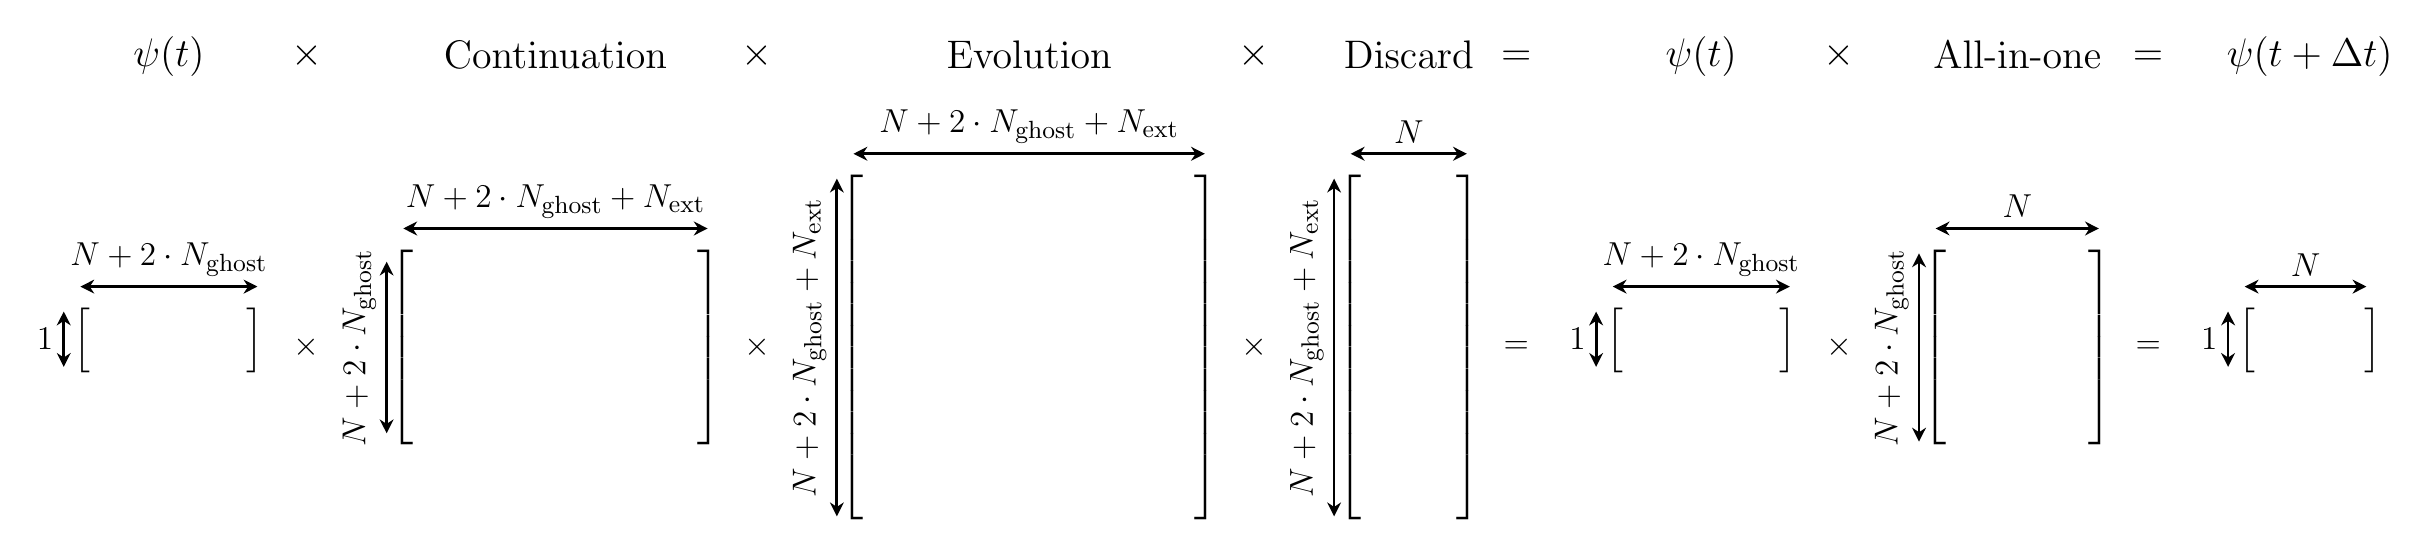
\begin{tikzpicture}[
    >={Stealth[length=5pt,width=5pt]},
    line width=1pt,
    every node/.style={font=\fontsize{13}{14.4}\selectfont},  % Adjust font size here
    node distance=1.5cm,
    every left delimiter/.style={xshift=1em},
    every right delimiter/.style={xshift=-1em},
    dimension/.style={decorate, decoration={brace, amplitude=5pt, raise=1pt}, line width=1pt, draw}
]

% Styles for matrices and vectors
\tikzset{
    matrixstyle/.style={
        matrix of math nodes,
        left delimiter={[},
        right delimiter={]},
        nodes in empty cells,
        minimum height=25pt,
        minimum width=15pt,
        inner sep=5pt,
        outer sep=5pt,
        nodes={draw=none, anchor=center, inner sep=5pt, outer sep=5pt},
        column sep=2pt,
        row sep=2pt,
    },
    vectorstyle/.style={
        matrix of math nodes,
        left delimiter={[},
        right delimiter={]},
        nodes in empty cells,
        minimum width=15pt,
        inner sep=2pt,  % Reduced from 5pt
        outer sep=2pt,  % Reduced from 5pt
        nodes={draw=none, minimum height=10pt, anchor=center, inner sep=5pt, outer sep=5pt}, % Reduced minimum height
        column sep=2pt,
        row sep=0pt, % Reduced row separation
    }
}
% Matrix A (NxM)
\matrix[matrixstyle] (A) {
    & & & & &\\
    & & & & &\\
};

% Vector x (size N)
\matrix[vectorstyle, left=of A] (x) {
    & & &\\
};

% Matrix B (MxP)
\matrix[matrixstyle, right=of A] (B) {
    & & & & & &\\
    & & & & & &\\
    & & & & & &\\
    & & & & & &\\
};

% Matrix C (PxQ)
\matrix[matrixstyle, right=of B] (C) {
    & \\
    & \\
    & \\
    & \\
};

% Vector x (size N)
\matrix[vectorstyle, right=of C] (x2) {
    & & &\\
};

% Matrix D (NxQ), product of A, B, and C
\matrix[matrixstyle, right=of x2] (D) {
    & & \\
    & & \\
};

% Vector b (size Q)
\matrix[vectorstyle, right=of D] (b) {
    & & \\
};


% Equation symbols
% Adjusting node distances individually
\node at ($(x.east)!0.5!(A.west) - (0.3cm, 0)$) (times1) {$\times$}; % Reduce space before A
\node at ($(A.east)!0.5!(B.west) - (0.3cm, 0)$) (times2) {$\times$}; % Reduce space before B
\node at ($(B.east)!0.5!(C.west) - (0.3cm, 0)$) (times3) {$\times$}; % Reduce space before C

\node at ($(C.east)!0.5!(x2.west) - (0.3cm, 0)$) (equals1) {$=$};
\node at ($(x2.east)!0.5!(D.west) - (0.3cm, 0)$) (times4) {$\times$};
\node at ($(D.east)!0.5!(b.west) - (0.3cm, 0)$) (equals2) {$=$};


% Dimension arrows
% Vector x (now 1 row × 3 columns)
\draw[<->] ([yshift=12pt, xshift=6pt]x-1-1.north west) -- node[above] {$N+2\cdot N_{\text{ghost}}$} ([yshift=12pt, xshift=-6pt]x-1-4.north east);% --- Horizontal (top) arrows for the transposed matrices/vectors ---

% Matrix A (now 2 rows × 6 columns)
\draw[<->] ([yshift=12pt]A-1-1.north west) -- node[above] {$N+2\cdot N_{\text{ghost}}+N_{\text{ext}}$} ([yshift=12pt]A-1-6.north east);

% Matrix B (now 4 rows × 7 columns)
\draw[<->] ([yshift=12pt]B-1-1.north west) -- node[above] {$N+2\cdot N_{\text{ghost}}+N_{\text{ext}}$} ([yshift=12pt]B-1-7.north east);

% Matrix C (now 4 rows × 2 columns)
\draw[<->] ([yshift=12pt]C-1-1.north west) -- node[above] {$N$} ([yshift=12pt]C-1-2.north east);

% Vector x2 (now 1 row × 4 columns)
\draw[<->] ([yshift=12pt, xshift=6pt]x2-1-1.north west) -- node[above] {$N+2\cdot N_{\text{ghost}}$} ([yshift=12pt, xshift=-6pt]x2-1-4.north east);

% Matrix D (now 2 row × 2 columns)
\draw[<->] ([yshift=12pt]D-1-1.north west) -- node[above] {$N$} ([yshift=12pt]D-1-3.north east);

% Vector b (now 1 row × 3 columns)
\draw[<->] ([yshift=12pt, xshift=6pt]b-1-1.north west) -- node[above] {$N$} ([yshift=12pt, xshift=-3pt, xshift=-6pt]b-1-3.north east);

% --- Vertical (side) arrows for the transposed matrices/vectors ---

% Vector x (now a row vector: 1 row × 4 columns)
\draw[<->] ([xshift=0pt, yshift=3pt]x-1-1.north west) -- node[left] {$1$} ([xshift=0pt, yshift=3pt]x-1-1.south west);

% Matrix A vertical (2 rows)
\draw[<->] ([xshift=-6pt]A-1-1.north west) -- node[rotate=90, above] {$N+2\cdot N_{\text{ghost}}$} ([xshift=-6pt]A-2-1.south west);

% Matrix B vertical (4 rows)
\draw[<->] ([xshift=-6pt, yshift=3pt]B-1-1.north west) -- node[rotate=90, above] {$N+2\cdot N_{\text{ghost}}+N_{\text{ext}}$} ([xshift=-6pt, yshift=-3pt]B-4-1.south west);

% Matrix C vertical (4 rows)
\draw[<->] ([xshift=-6pt, yshift=3pt]C-1-1.north west) -- node[rotate=90, above] {$N+2\cdot N_{\text{ghost}}+N_{\text{ext}}$} ([xshift=-6pt, yshift=-3pt]C-4-1.south west);

% Vector x2 vertical (1 row)
\draw[<->] ([xshift=0pt, yshift=3pt]x2-1-1.north west) -- node[left] {$1$} ([xshift=0pt, yshift=3pt]x2-1-1.south west);

% Matrix D vertical (2 rows)
\draw[<->] ([xshift=-6pt, yshift=3pt]D-1-1.north west) -- node[rotate=90, above] {$N+2\cdot N_{\text{ghost}}$} ([xshift=-6pt, yshift=-3pt]D-2-1.south west);

% Vector b vertical (1 row)
\draw[<->] ([xshift=0pt, yshift=3pt]b-1-1.north west) -- node[left] {$1$} ([xshift=0pt, yshift=3pt]b-1-1.south west);



% Labels for vectors and matrices

\pgfmathsetlengthmacro{\offset}{-7pt} % Change this to shift up/down

\node[above= {\dimexpr 92pt + \offset} of x] {\Large $\psi(t)$};
\node[above= {\dimexpr 96pt + \offset} of times1] {\Large $\times$};
\node[above= {\dimexpr 68pt + \offset} of A] {\Large Continuation};
\node[above= {\dimexpr 96pt + \offset} of times2] {\Large $\times$};
\node[above= {\dimexpr 41pt + \offset} of B] {\Large Evolution};
\node[above= {\dimexpr 96pt + \offset} of times3] {\Large $\times$};
\node[above= {\dimexpr 41pt + \offset} of C] {\Large Discard};
\node[above= {\dimexpr 99pt + \offset} of equals1] {\Large $=$};
\node[above= {\dimexpr 92pt + \offset} of x2] {\Large $\psi(t)$};
\node[above= {\dimexpr 96pt + \offset} of times4] {\Large $\times$};
\node[above= {\dimexpr 68pt + \offset} of D] {\Large All-in-one};
\node[above= {\dimexpr 99pt + \offset} of equals2] {\Large $=$};
\node[above= {\dimexpr 92pt + \offset} of b] {\Large $\psi(t+\Delta t)$};



\end{tikzpicture}


\end{document}
